% !TEX TS-program = xelatex
\documentclass[a4paper, 10pt]{article}
\usepackage{a4wide}
%\usepackage[T1]{fontenc}
\usepackage[utf8]{inputenc}
\usepackage[spanish]{babel}
\usepackage[none]{hyphenat}
\usepackage{xltxtra,fontspec,xunicode}
\setromanfont[Numbers=Uppercase]{Helvetica Light}
\usepackage{hyperref}
\usepackage[top=40pt,bottom=50pt,left=48pt,right=46pt]{geometry}
\usepackage{tabularx}
\usepackage{enumitem}
\usepackage{titling}
\usepackage{multicol}
\usepackage{graphicx}
\usepackage{color}
\usepackage{xcolor}
\usepackage{framed}
\usepackage{tikz}
\usepackage{scrextend}
\usepackage{wrapfig}
\usepackage{float}
\usepackage{calc}


\usetikzlibrary{decorations.pathreplacing}
\usetikzlibrary{shadows}
\usetikzlibrary{calc}

\definecolor{darkgray}{HTML}{3C3C3C}
\definecolor{lightgray}{HTML}{6C6C6C}


\newcommand{\CVSection}[1]{ {\setromanfont[Numbers=Uppercase]{Helvetica}\selectfont \section*{#1}} }
\newcommand{\CVSubsection}[1]{ {\setromanfont[Numbers=Uppercase]{Helvetica}\selectfont \subsection*{#1}} }
\newcommand{\CVComment}[1]{{\fontsize{0.75em}{1em}\selectfont #1}}

%\titleformat{\section}{\large\bfseries\setromanfont[Numbers=Uppercase]{Corbel}\selectfont}{}{0pt}{\thesection}

\renewenvironment{leftbar}[1][\hsize]
{%
    \def\FrameCommand
    {%
        {\color{darkgray}\vrule width 2pt}%
        %\hspace{0pt}%must no space.
        %\fboxsep=\FrameSep\colorbox{yellow}%
    }%
    \MakeFramed{\hsize#1\advance\hsize-\width\FrameRestore}%
}
{\endMakeFramed}

\makeatletter
\newcommand{\gettikzxy}[3]{%
  \tikz@scan@one@point\pgfutil@firstofone#1\relax
  \edef#2{\the\pgf@x}%
  \edef#3{\the\pgf@y}%
}
\makeatother

\newenvironment{timeline}{
	\begin{leftbar}
}{
	\end{leftbar}
}

\setlength\parindent{0pt}

\newenvironment{job}[1][date]{
	\newcommand{\jobdate}{#1}
	\vspace{10pt}
	\begin{addmargin}[4\parindent]{0pt}
	\begin{minipage}{\linewidth}
	\tikz[remember picture] \node[coordinate,yshift=0.5em] (start) {};
}{
	\tikz[remember picture] \node[coordinate] (end) {};
	%\xdef\tpd{\the\prevdepth}
	\end{minipage}
	\end{addmargin}

	\begin{tikzpicture}[overlay,remember picture]

		\pgfmathsetmacro\triangleLength{0.4}
		\pgfmathsetmacro\halfTriangleLength{(\triangleLength/2)}

		\gettikzxy{(start)}{\startx}{\starty}
		\gettikzxy{(end)}{\endx}{\endy}

		\node[coordinate] (start) at (\startx-10pt,\starty) {};
		\node[coordinate] (end) at (\startx-10pt,\endy-5pt) {};

		\node[coordinate] (middle) at ($(start)!0.5!(end)$) {};

		\node[coordinate] (triangle-up) at ($(middle) + (0, \halfTriangleLength)$) {};
		\node[coordinate] (triangle-down) at ($(middle) + (0, -\halfTriangleLength)$) {};
		\node[coordinate] (triangle-tip) at ($(middle) + (-\halfTriangleLength, 0)$) {};

		\draw[thick, lightgray]
			(start) -- (triangle-up) -- (triangle-tip) -- (triangle-down) -- (end);

		\node (date) at (triangle-tip) [left, text width=1cm, align=center] {\jobdate};

		%\foreach \xy in {start, triangle-up, triangle-down, end}{
 		%   \node at (\xy) {\xy};
		%}

  	\end{tikzpicture}
  	\vspace{10pt}
}





\def\shadowshift{3.5pt,-3.5pt}
\def\shadowradius{2pt}

\colorlet{innercolor}{gray!30}
\colorlet{outercolor}{gray!01}

% this draws a shadow under a rectangle node
\newcommand\drawshadow[1]{
    \begin{pgfonlayer}{shadow}
        \shade[outercolor,inner color=innercolor,outer color=outercolor] ($(#1.south west)+(\shadowshift)+(\shadowradius/2,\shadowradius/2)$) circle (\shadowradius);
        \shade[outercolor,inner color=innercolor,outer color=outercolor] ($(#1.north west)+(\shadowshift)+(\shadowradius/2,-\shadowradius/2)$) circle (\shadowradius);
        \shade[outercolor,inner color=innercolor,outer color=outercolor] ($(#1.south east)+(\shadowshift)+(-\shadowradius/2,\shadowradius/2)$) circle (\shadowradius);
        \shade[outercolor,inner color=innercolor,outer color=outercolor] ($(#1.north east)+(\shadowshift)+(-\shadowradius/2,-\shadowradius/2)$) circle (\shadowradius);
        \shade[top color=innercolor,bottom color=outercolor] ($(#1.south west)+(\shadowshift)+(\shadowradius/2,-\shadowradius/2)$) rectangle ($(#1.south east)+(\shadowshift)+(-\shadowradius/2,\shadowradius/2)$);
        \shade[left color=innercolor,right color=outercolor] ($(#1.south east)+(\shadowshift)+(-\shadowradius/2,\shadowradius/2)$) rectangle ($(#1.north east)+(\shadowshift)+(\shadowradius/2,-\shadowradius/2)$);
        \shade[bottom color=innercolor,top color=outercolor] ($(#1.north west)+(\shadowshift)+(\shadowradius/2,-\shadowradius/2)$) rectangle ($(#1.north east)+(\shadowshift)+(-\shadowradius/2,\shadowradius/2)$);
        \shade[outercolor,right color=innercolor,left color=outercolor] ($(#1.south west)+(\shadowshift)+(-\shadowradius/2,\shadowradius/2)$) rectangle ($(#1.north west)+(\shadowshift)+(\shadowradius/2,-\shadowradius/2)$);
        \filldraw[color=innercolor] ($(#1.south west)+(\shadowshift)+(\shadowradius/2,\shadowradius/2)$) rectangle ($(#1.north east)+(\shadowshift)-(\shadowradius/2,\shadowradius/2)$);
    \end{pgfonlayer}
}

% create a shadow layer, so that we don't need to worry about overdrawing other things
\pgfdeclarelayer{shadow} 
\pgfsetlayers{shadow,main}


\newcommand\shadowimage[2][]{%
\begin{tikzpicture}
\node[anchor=south west,inner sep=0] (image) at (0,0) {\includegraphics[#1]{#2}};
\drawshadow{image}
\end{tikzpicture}}



\pagenumbering{gobble}




\begin{document}

%\begin{minipage}
  \begin{minipage}{0.25\linewidth}   

  	\vspace{100pt}
  	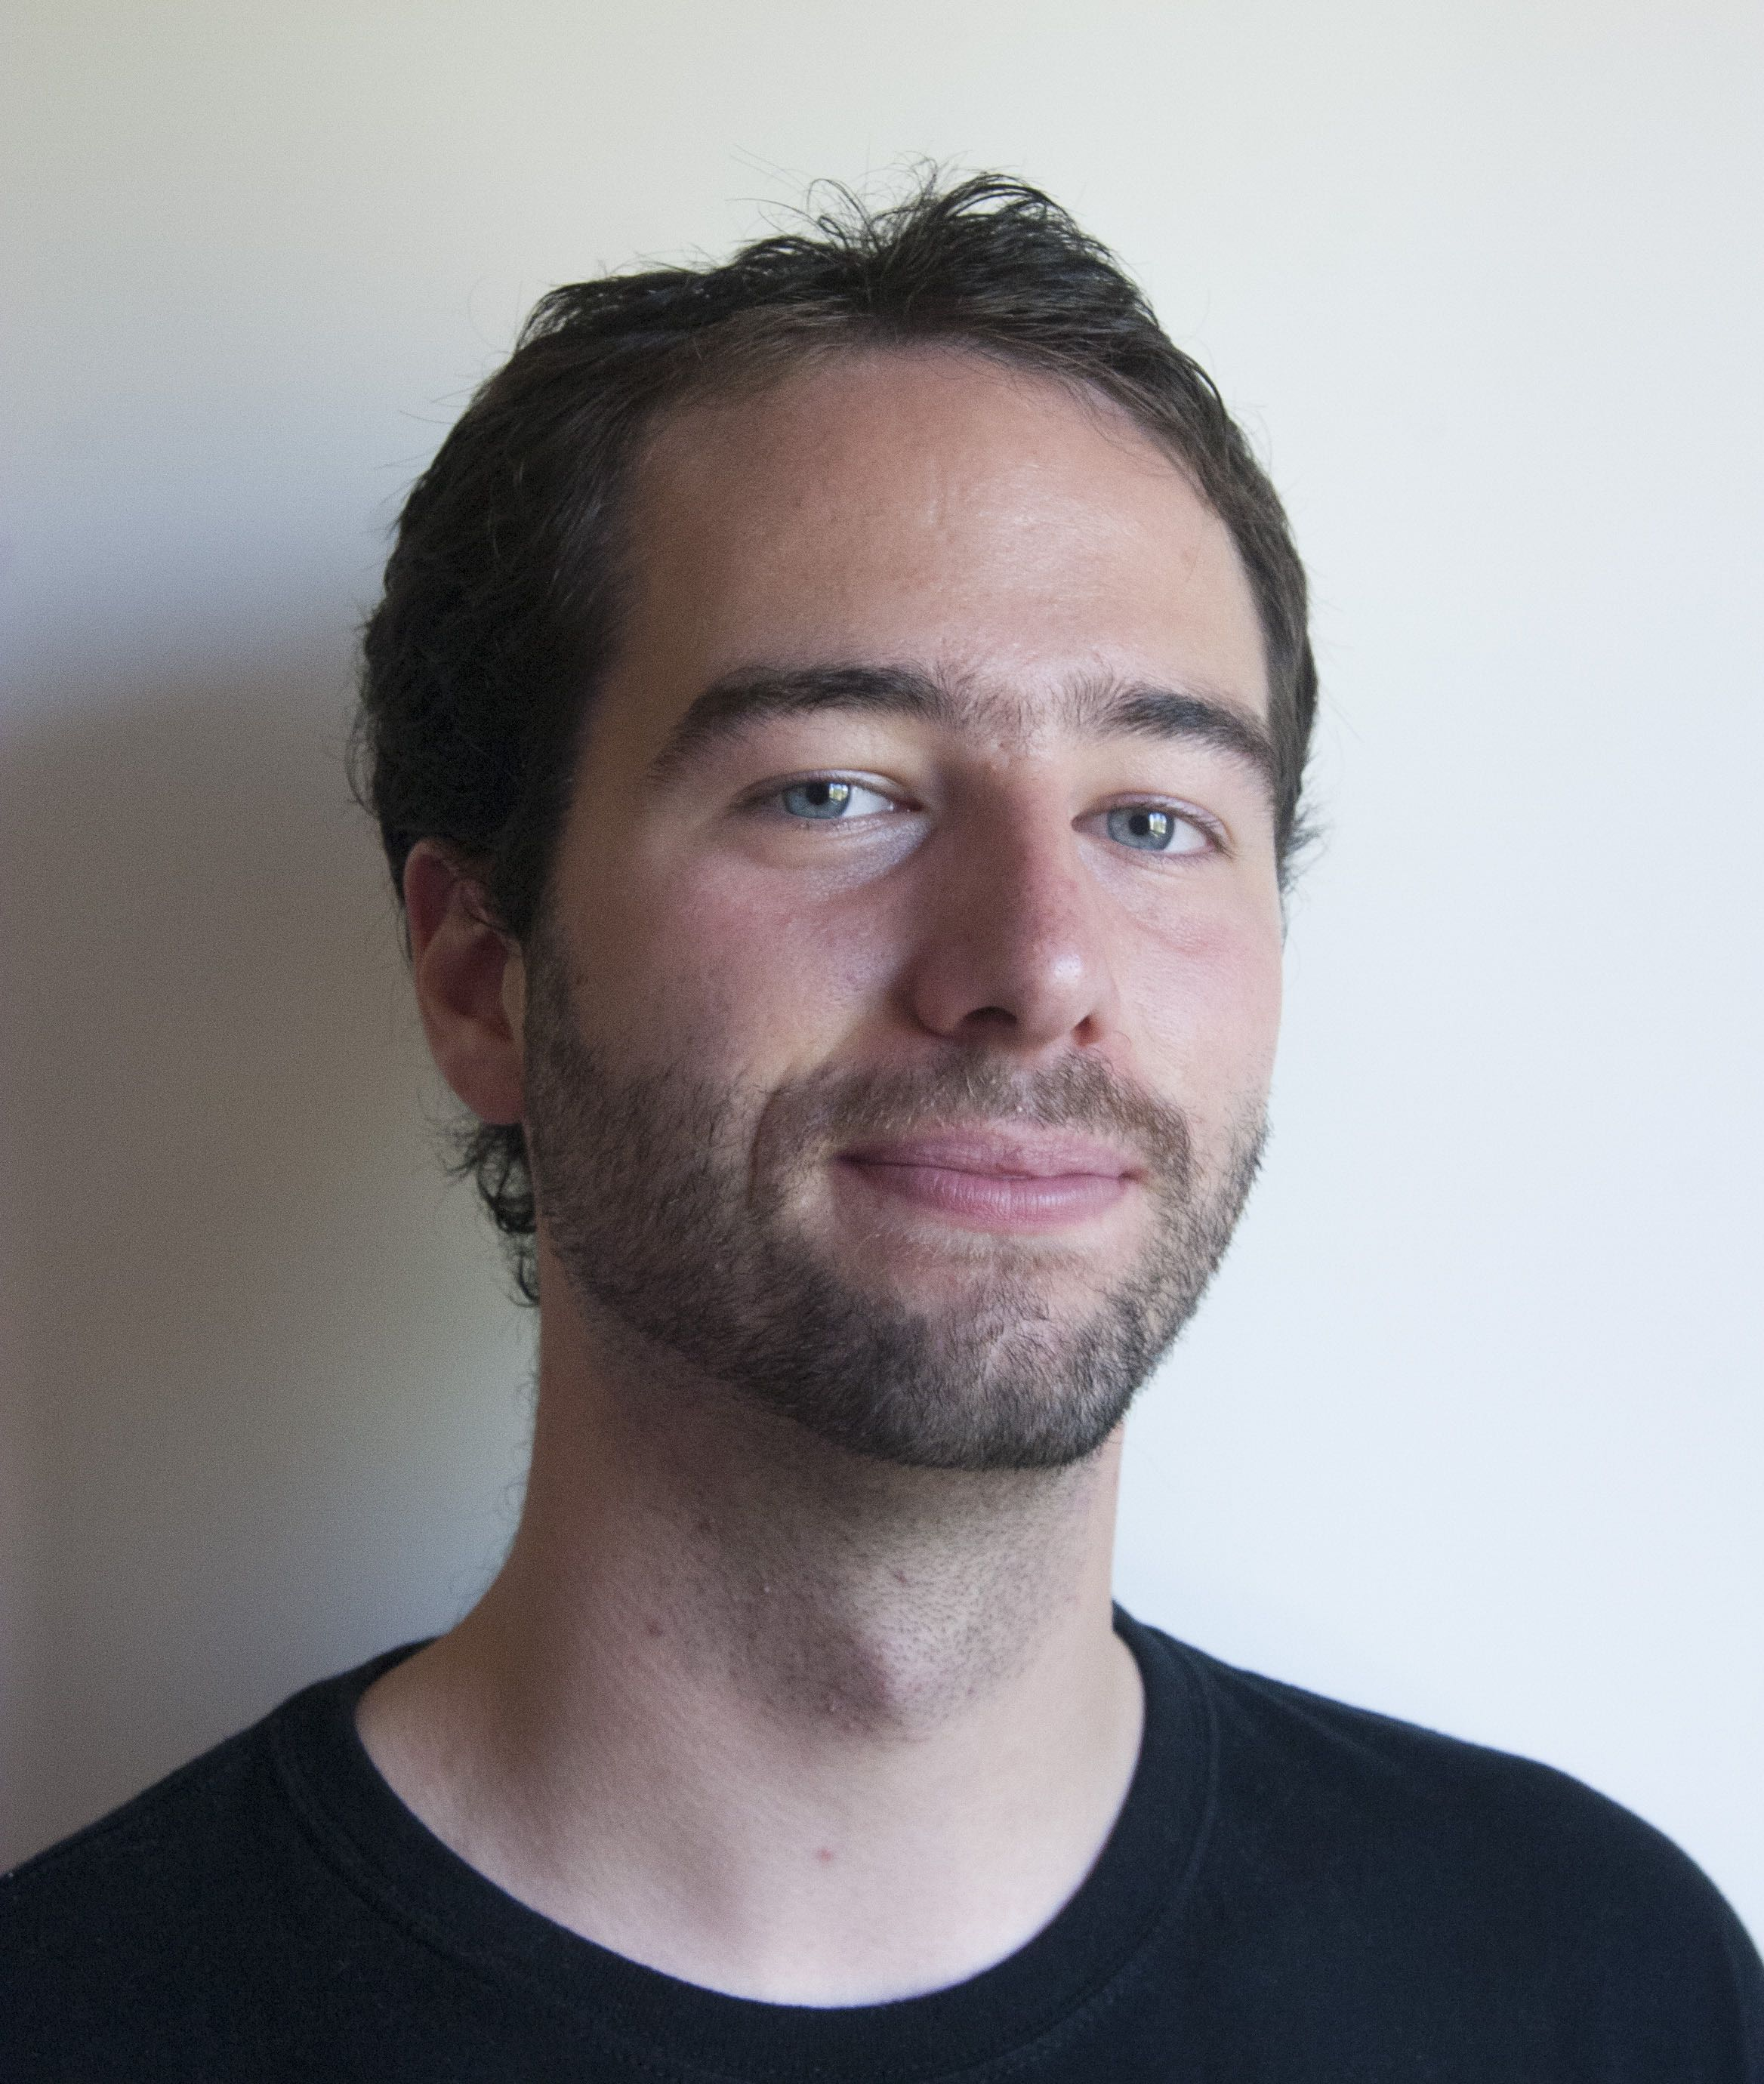
\includegraphics[width=0.23\linewidth]{images/me.jpg}

  \end{minipage}
  \begin{minipage}{0.75\linewidth}

  	\begin{flushright}

  		\vspace{-35pt}

	  	{\setromanfont[Numbers=Uppercase]{Corbel}\selectfont {\fontsize{4em}{1em}\selectfont Guillermo Guridi}}

	  	\vspace{25pt}

		{\setromanfont[Numbers=Uppercase]{Helvetica Light}\selectfont

			{\fontsize{1.6em}{2em}\selectfont Estudiante de Matemáticas e Informática en la UAM

			Desarrollador de páginas web (frontend y backend)

			
			}
		}

	\end{flushright}

  \end{minipage}
%\end{minipage}

\vspace{-10mm}
\begin{flushright}
\CVSection{Conocimientos}

\end{flushright}

A parte de las competencias básicas adquiridas en la carrera he complementado mis estudios con cursos online, pequeños trabajos y otros proyectos personales que me han llevado a aprender mucho más.


\begin{multicols}{2}

		\CVSubsection{Cursos online completados}
		\vspace{-6mm}
		\CVComment{en Coursera, Udacity y otros.}





		\begin{itemize}
			\item Machine Learning (2011)

			\item Introduction to databases (2011)

			\item Introduction to AI (2011) \\ and AI for robotics (2012)

			\item Sw. engineering for SaaS (2012)

			\item Criptography (2012)

			\item Cisco Network Fundamentals (2013)

		\end{itemize}

		\columnbreak

		\CVSubsection{Lenguajes de programación}
		\vspace{-4mm}
		\CVComment{y algunos frameworks.}

		
\includegraphics[width=0.9\linewidth]{images/languages.png}

\end{multicols}

\CVSubsection{Tecnologías}

\begin{multicols}{2}
	
	\begin{itemize}

		\item He trabajado con y desarrollado aplicaciones para iOS y OS X.

		\item Estoy familiarizado con entornos GNU Linux, tanto a nivel usuario como administrador. He desplegado servidores en Amazon AWS usando Docker, Apache, MySQL, Postgres, Ruby on Rails, CouchDB...

		\item Tengo experiencia en el uso de programas de diseño gráfico como Adobe Photoshop

		\item He trabajado con sistemas integrados como RaspberryPi o Arduino

		\item Uso git como sistema de control de versiones en mi día a día.


	\end{itemize}

\end{multicols}

\CVSubsection{Idiomas}

El \textbf{español} es mi lengua materna, tengo un nivel casi nativo de \textbf{ingés} tanto oral como escrito, y soy un principiante en \textbf{francés} y \textbf{sueco} aunque me gustaría aprender más.


\begin{huge}
	Soy una persona realmente apasionada por lo que hace. Disfruto mucho con toda clase de problemas matemáticos e informáticos y me encantan los retos. No me importa trabajar individualmente pero prefiero el trabajo en equipo.
\end{huge}

%\begin{enumerate}
%	\begin{minipage}
%
%	\end{minipage}
%	\begin{minipage}
%
%	\end{minipage}
%\end{enumerate}



\pagebreak


Born late 1993

\begin{timeline}

\begin{job}[2012 \\- \\ 2013]

	adwa
	awoidjwa
	dawdaw
	daw

	d
	wadwad
	wa
	d

	wadwadwa

	sad
	asdasd


	adsasdasda
	daw
	daw
	aw


	qweqweqw
	eqweqewqeq
\end{job}


\begin{job}
	
		\begin{wrapfigure}{l}{0.3\textwidth}
			\vspace{-5pt}
			\begin{center}
				
\includegraphics[width=0.3\textwidth]{images/2cs.png}	
			\end{center}
			\vspace{-5pt}
		\end{wrapfigure}
		oaijda oaiwjd adoeijd aeodijae doaeidj aeoidjae daeoidjaeoidjae doiajed aeoidja edoiajed aoiedj aodijae doaiejd aeodijaeodi aeoidja edoiajd aiurfha rogua rifuahrf asiurfh saiufh sairfhas ruifh sirufhsi urfh siuf sriu fhsiurhfisruf siuhfs riufhsiurf ahrisfuhaaiua ciuhc siuchsr icusrhic sruhc irsuhc riuhiuhc sruchisruhc irsuhrciushrc isurhc siruch sriuch siuhc isu ciusr ciurs icushriuc hsriuchsriuhs ruhcis uchsr u sr ciusiuhcsiu. aowidjaw doaiwd awodjaw odiawj doawijdawj.daw doaijwda.dawidjaow diaowidj aowdj aowid aeoijd aeoidj aed.aed oaeidoae daeoidae daedhae da edae diuhaed iaued iauehd aeiudh aieudh aieud aieudhae iud aeid.a eodia edo aoied oai eodijaoied aeoidj aeoid ae.
\end{job}

\begin{job}
	awoidjwa
	dawdaw
	daw

	d
	wadwad
	wa
	d

	wadwadwa

	sad
	asdasd


	adsasdasda
	daw
	daw
	aw


	qweqweqw
	eqweqewqeq
\end{job}

\begin{job}
	awoidjwa
	dawdaw
	daw

	d
	wadwad
	wa
	d

	wadwadwa
\end{job}

\end{timeline}


%\textcolor{darkgray}{\rule{2pt}{26cm}}


\end{document}
